%%
%% Copyright 2007, 2008, 2009 Elsevier Ltd
%%
%% This file is part of the 'Elsarticle Bundle'.
%% ---------------------------------------------
%%
%% It may be distributed under the conditions of the LaTeX Project Public
%% License, either version 1.2 of this license or (at your option) any
%% later version.  The latest version of this license is in
%%    http://www.latex-project.org/lppl.txt
%% and version 1.2 or later is part of all distributions of LaTeX
%% version 1999/12/01 or later.
%%
%% The list of all files belonging to the 'Elsarticle Bundle' is
%% given in the file `manifest.txt'.
%%

%% Template article for Elsevier's document class `elsarticle'
%% with numbered style bibliographic references
%% SP 2008/03/01
%%
%%
%%
%% $Id: elsarticle-template-num.tex 4 2009-10-24 08:22:58Z rishi $
%%
%%
\documentclass[preprint,review,10pt,3p]{elsarticle}

%% Use the option review to obtain double line spacing
%% \documentclass[preprint,review,12pt]{elsarticle}

%% Use the options 1p,twocolumn; 3p; 3p,twocolumn; 5p; or 5p,twocolumn
%% for a journal layout:
%% \documentclass[final,1p,times]{elsarticle}
%% \documentclass[final,1p,times,twocolumn]{elsarticle}
%% \documentclass[final,3p,times]{elsarticle}
%% \documentclass[final,3p,times,twocolumn]{elsarticle}
%% \documentclass[final,5p,times]{elsarticle}
%% \documentclass[final,5p,times,twocolumn]{elsarticle}

%% if you use PostScript figures in your article
%% use the graphics package for simple commands
%% \usepackage{graphics}
%% or use the graphicx package for more complicated commands
\usepackage{graphicx}
%% or use the epsfig package if you prefer to use the old commands
%% \usepackage{epsfig}

\usepackage{subfigure}
\usepackage[linesnumbered,ruled, boxed]{algorithm2e}

%% The amssymb package provides various useful mathematical symbols
\usepackage{amssymb}
%% The amsthm package provides extended theorem environments
%% \usepackage{amsthm}

%% The lineno packages adds line numbers. Start line numbering with
%% \begin{linenumbers}, end it with \end{linenumbers}. Or switch it on
%% for the whole article with \linenumbers after \end{frontmatter}.
%% \usepackage{lineno}

%% natbib.sty is loaded by default. However, natbib options can be
%% provided with \biboptions{...} command. Following options are
%% valid:

%%   round  -  round parentheses are used (default)
%%   square -  square brackets are used   [option]
%%   curly  -  curly braces are used      {option}
%%   angle  -  angle brackets are used    <option>
%%   semicolon  -  multiple citations separated by semi-colon
%%   colon  - same as semicolon, an earlier confusion
%%   comma  -  separated by comma
%%   numbers-  selects numerical citations
%%   super  -  numerical citations as superscripts
%%   sort   -  sorts multiple citations according to order in ref. list
%%   sort&compress   -  like sort, but also compresses numerical citations
%%   compress - compresses without sorting
%%
%% \biboptions{comma,round}

% \biboptions{}


\journal{IPL}


\begin{document}

\begin{frontmatter}


%\mainmatter  % start of an individual contribution

% first the title is needed
\title{Gradient Boosting to Precompute Multiple Signals in Search Index Construction}

\author[mymainaddress]{Sheila N{\'obrega}}
\author[mymainaddress]{Edleno Moura}
\author[mysecondaryaddress]{P{\'a}vel Calado}
\author[mymainaddress]{Altigran Silva}

\address[mymainaddress]{Universidade Federal do Amazonas, Brasil}
\address[mysecondaryaddress]{INESC-ID, Instituto Superior T{\'e}cnico, Universidade de Lisboa}

\begin{abstract}

%There has been an ongoing effort to apply \textit{learning to rank} techniques in search engines query processing, with the goal of enhancing the quality of the search results. Most works, however, focus on applying such techniques at query time, thus adding complexity to the search process. 
In this paper we address the problem of using a learning to rank technique to fuse sources of relevance evidence at indexing time. We propose to use a modified Gradient Boosted Regression Tree algorithm to generate \textit{unified term impacts} (UTI) to be stored in the index.
% The UTI is the only value needed later for ranking the documents, thus greatly reducing the effort needed to compute the document scores. 
Our approach achieves better results in quality, when compared to previously proposed methods to compute UTI, and greatly reduces the time required for training. In addition, we show how to obtain significant gains in index compression with virtually no loss in the final quality of results.
% This is achieved by exploiting a simple, yet effective, reduction of size in the representation of the unified term impact values, when the inverted list is created. 
%Our best approach was able to achieve 91\% compression rate of the index, while keeping the quality of results on par with methods that do not use compression.


\begin{keyword}
\texttt Learning to Rank \sep Search Engines \sep Indexing \sep LambdaMART \sep Gradient Boosting
\end{keyword}

\end{abstract}
\end{frontmatter}


%%
%% Start line numbering here if you want
%%
% \linenumbers

%% main text

\section{Introduction}
\label{intro}

The production of high quality ranking results for their users is a fundamental aspect of Web search engines. Users expect the answers to their queries to be shown at the top of the list and rarely tend to go beyond the first page displayed~\cite{saraiva2001rank}. 
%When unsatisfied, in the best case, users will issue new queries, thus increasing the load of the system, while in the worst case, they will simply try a competitor system. 
Further, modern search engine users are used to experience fast query processing times, regardless of the size of the dataset, and any noticeable increase in waiting time can be a fatal blow to the their perception of the quality of the system. Thus, although commercial search engines can receive tens of thousands of queries per second, each one requiring access to a massive collection of data, computational efficiency cannot be obtained at the cost of quality. 

The issue of quality is usually addressed through a class of machine learning techniques commonly known as \textit{learning to rank} (L2R). Query processing by a L2R-based search engine is performed in two steps: first, the top-k documents for a query are retrieved using a low cost ranking strategy,  referred to as base ranker, such as BM25; second, the documents are re-ranked with the more expensive L2R model, referred to as top-ranker˜\cite{capannini2016quality}.

An important aspect of modern search engines is the use of a large number of distinct sources of relevance evidence to build the L2R model. Relevance evidence can be defined as the set of features that can be extracted from the documents, which collectively make the document relevant to the query issued by the user. Examples of such sources of relevance evidence are frequencies of terms in text, urls, titles, and other parts of the document
%, part of speech tags
, web link graph analysis
%, anchor text of the incoming links to a web page, HTML structure, such as titles and headings, url tokenization
, among others~\cite{baezaribeiro2011modinforet}. 

%These distinct sources of relevance evidence are used to compute the query result rankings. 
%The query result rankings is computed by fusing all sources into a single document score, for each document in the final ranking. In the past few decades, most work on fusing evidence has been done with the deployment of L2R methods such as RankBoost~\cite{freund2003efficient}, Genetic Programming based methods~\cite{de2007combined, silva2009evolutionary}, RankSVM~\cite{joachims2002optimizing} and, the current state of the art, Gradient Boosting method LambdaMART~\cite{wu2010lambdamart}. These methods use examples of queries and their respective results, to train a supervised learning model that determines the relative position of the documents in the result list. Once trained, the model can be used during query processing to determine the final ranking. This approach, however, inadvertently adds computational costs to query processing, which may lead to a drop in time  performance.

The query result rankings is computed by fusing all sources into a single document score, for each document in the final ranking. In the past few decades, most work on fusing evidence has been done with the deployment of L2R methods, such as  Gradient Boosting method LambdaMART~\cite{wu2010lambdamart}, which is now among the current state- of-art methods. L2R methods use examples of queries and their respective results, to train a supervised learning model that determines the relative position of the documents in the result list. Once trained, the model can be used during query processing to determine the final ranking. This approach, however, inadvertently adds computational costs to query processing, which may lead to a drop in time  performance.


\newcommand{\lepref}{LePrEF}
\newcommand{\lambdamart}{LambdaMART}

To mitigate this problem, an alternative approach has been proposed --- Learn to Precompute Evidence Fusion (\lepref)~\cite{costa2012lepref}, also based on supervised learning. \lepref\ proposes to implement the bulk of the evidence fusion during indexing time, generating a single inverted index containing unified entries regarding all features, called \textit{Unified Term Impacts} (UTIs). 
%Fig.~\ref{fig:arq} shows a diagram of \lepref's architecture. 
%Contrary to traditional systems, the \lepref\ approach does not maintain separate inverted indexes for each source of relevance evidence. Instead, it creates a single inverted index containing the fused values for all sources, i.e. the UTIs. 
Each UTI is computed based on a trained L2R model and, at query time, the search engine needs only to add each of the query term's UTI to directly obtain the document scores.
We  propose and study here an adaptation of \lambdamart~\cite{wu2010lambdamart}, a gradient boosting algorithm, to compute the UTIs of each term at the indexing time. 
%\begin{figure}
%\begin{center}
%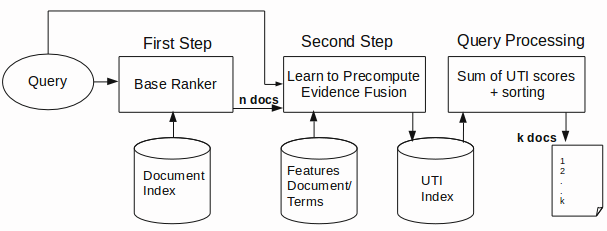
\includegraphics[width=12cm, height=5cm]{im_arquitetura.png}
%\caption{The LePrEF architecture. }
%\label{fig:arq}
%\end{center}
%\end{figure}



%While the authors of LePrEF show that it can lead to high quality results, they're approach has several drawbacks.  First, UTIs are computed using Genetic Programming~\cite{Koza97geneticprogramming}, an optimization method that has a high computational cost during the model training phase. Second, XXXXXX. In this work, we avoid these issues by proposing an adaptation of \lambdamart~\cite{wu2010lambdamart}, a gradient boosting algorithm, to compute the UTIs of each term at the indexing time. \lambdamart\ was designed specifically to optimize ranking quality metrics, such as NDCG, and was shown to be very effective in traditional (i.e. query-time) L2R tasks. Our adaptation allows to achieve results in 2.8\% of the time required by LePrEF using GP without lost of quality.



%Our adaptation allows for improvements in the quality of the rankings produced varying from XXXX through %XXXX points in precison, when compared to the state of the art. Also, we are able to achieve these results %in XXXX of the time required by LePref. 


The remaining  of this article is organized as follows: In Section~\ref{relatedwork}, we discuss related work and an overview of the basic concepts involved. Section ~\ref{lambda} presents the proposed method describing how we use LambdaMART to generate query term UTI scores in the indexing time. Section ~\ref{experiments} presents the experimental setup followed by experimental results in comparison to current baselines in Section~\ref{results}. Finally, Section~\ref{conclusion} presents the conclusive remarks and directions to future research.

\section{Related Work}
\label{relatedwork}

%Machine learning has been successfully adopted in a wide range of Information Retrieval applications, including in important components of search systems, such as query processing, classifying queries according to user goals, and indexing~\cite{costa2012lepref}. Here, we will focus on the latter case, i.e. using machine learning techniques to create search engine indexes.

%A key concept in any search engine architecture is the set of \emph{sources of relevance evidence adopted} for ranking query results. We define a source of relevance evidence as any information that can be extracted from the document collection to contribute to rank query answers according to the user's interest. For example, common sources of evidence used by Web search engines include the pages' content, anchor text, url text, title, image descriptions, among others. All these can be used to infer if a webpage is relevant to the user's query or not. This information is translated into numerical values that are either computed at query time, or stored in search engine indexes. Values computed at query time usually represent information that depends both on the query and the document, such as the TF-IDF term weight, the cosine similarity between the query and the document, etc. Values stored in inverted indexes usually represent information that depends only on the documents, such as the term frequency values, PageRank values, number of slashes in the URL etc. In this work, we are particularly interested in the later set of values, those that do not depend on the query. Our goal is to compute a combination of such values, which we designate as Unified Term Impact values (UTIs), and store them for later use, at query time.

The use of precomputed term impacts in documents was first proposed and studied by Anh and Moffat~\cite{Anh:2002:ITE:564376.564380}
%, and was further addressed in two other followup articles~\cite{Anh:2005:SSS:1076034.1076075,anh2008term}. 
Their work aimed to reduce the number of arithmetic computations performed at query processing times, using a fixed term impact computation strategy that was not based on machine learning. Carvalho et al~\cite{costa2012lepref} proposed a method, called \lepref, to precompute UTI values from multiple sources of relevance evidence, using Genetic Programming (GP)
%~\cite{Koza97geneticprogramming} 
 to fuse such sources into a single numerical value, at indexing time. 
%This method discards all features not readily available at indexing time and adopts the concept of a single numerical value to represent the whole set of sources of relevance evidences, both query dependent and query independent. 
%Such numerical values are named Unified Term Impact (UTI) values , and are stored in the inverted index to be used at query processing time. 
This method makes query processing faster, at the cost of increased computational costs during indexing. In fact, although the authors showed that learning to precompute evidence fusion is a promising strategy, the long time required to train the evidence fusion model was a major hindrance. 

We  here propose an adaptation of \lambdamart~\cite{wu2010lambdamart}, a gradient boosting algorithm, to compute the UTIs of each term at the indexing time. \lambdamart\ was designed specifically to optimize ranking quality metrics, such as NDCG, and was shown to be very effective in traditional (i.e. query-time) L2R tasks. We show experiments where  our adaptation of \lambdamart achieves results in 2.8\% of the time required by \lepref using GP without lost of quality. Further, the use of UTI with \lambdamart produces results on pair with the ones produced by state-of-art learning to rank methods.

In here, we improve the work done on \lepref\ in three ways. First, we significantly reduce the required training time. Second, by carefully tuning the algorithm, we are able to achieve higher quality search results. Finally, using a simple compression procedure, we are able to greatly reduce the space requirements of the inverted index, without any significant loss in search quality. In the remainder of this text, we refer this 
proposed approach as UTI-LambdaMART. We present experiments to compare the performance of UTI-LambdaMART with UTI using GP.

The issues related to combining efficiency and effectiveness in learning to rank have been recently addressed in the literature. Chen et al.~\cite{Chen2017} study  the importance of tightly integrating feature costs into multi-stage L2R IR systems. They present an approach to optimize cascaded ranking models  which provides a better balance between efficiency and quality of ranking results.  The study proposed here can be combined with the cascade strategy proposed by them, since the UTI approaches can be  incorporated in any cascade ranking strategy.

Lucchese et al.~\cite{Lucchese2016}  propose a  framework, named CLEaVER, for optimizing  learning to ranking models based on ensembles of regression trees.  Their method first removes a subset of the trees in the ensemble, and then fine-tunes the weights of the remaining trees according to any given quality measure. Experiments conducted on two publicly available  datasets show that CLEaVER is able to prune up to 80\% of the trees. Again, their method is orthogonal to the ones proposed here. Their pruning strategy can be also applied when fusing evidences at indexing times, which may further reduce the computational costs  of training. 


%LambdaMART~\cite{wu2010lambdamart} is a gradient boosting algorithm that has been used with success in many different machine learning scenarios. We %choose to use this algorithm to LePrEF using a method that can be adopted by a real search engine considering its fast performance in the training and %test phases when compared  to GP. Further,  previous research on L2R methods indicate that LambdaMART achieves  better quality results in ranking  %when compared to L2R using GP. 




\section{The modified \lambdamart\ Algorithm}
\label{lambda}
\newcommand{\lamdamart}{LambdaMART}

The \lambdamart\ algorithm~\cite{wu2010lambdamart} is a combination of
MART~\cite{Jerome2001}, a L2R method that adopts a boosted tree model, and LambdaRank~\cite{Burges2006},
another L2R method that adopts a neural network model. It is
particularly interesting for our work since it allows us to directly
optimize a rank quality measure, such as precision or NDCG. We will
now present a brief explanation of the points necessary to understand
how to use LambdaMART to generate UTIs (Unified Term Impact).

LambdaMART constructs the ranking model $F(x=(q,d,r_d,fs_{(d,q)}))$,
$x$ is a tuple composed of $q$, which is a query, $d$ which is a
document number, $r_d \in \{0,1,2\}$ which defines the relevance level of
$d$ as an answer to $q$ and of $fs_{(d,q)}$, which denotes the set of
feature values related to document $d$ and query $q$. Model $F$ maps
each training instance $x$ into a numerical score $F(x)$.

Although based on \lambdamart, our approach computes one model $Ft$
to each query term, instead of computing a single model to the whole
query. Thus, in our case, each instance $x=(q,d,r_d,fs_{(d,q)})$ is
decomposed into $|q|$ training instances in the form $x_t=
(t,d,r_d,fs_{(d,t)}))$, where $t \in q$, and $fs_{(d,t)}$ denotes the
set of feature values related to document $d$ and term $t$. Notice
that query dependent features are not available in $x_t$, which makes
the number of features adopted by our model smaller than the ones
adopted in original \lambdamart. The model $Ft$ is trained and then
applied to compute the UTI values that we store at indexing times.

\begin{algorithm}[ht!]
\caption{Algorithm LambdaMART for Precomputing UTI }
\label{alg:utilambda}
\SetAlgoLined
\SetKwInOut{Input}{input}\SetKwInOut{Output}{output}
\Input{number of trees $N$, training instances set $\mathcal{M}$, number of levels per tree $L$}
\Output{Model to compute UTI values}
\ForEach{$(q,d,r_d,fs_{(d,q)}) \in \mathcal{M}$}{
    \lForEach{$t \in q$} {
        $Ft_0((t,d,r_d,fs_{(d,t)})) \leftarrow 0$ 
    }
}
\For{$n\leftarrow 1$ \KwTo $N$}{
    \ForEach{$(q,d,r_d,fs_{(d,q)}) \in \mathcal{M}$}{
        $scores[d,q] \gets 0$\;
        \lForEach{$t \in q$}{
           $scores[d,q] \gets scores[d,q] + Ft_{n-1}((t,d,r_d,fs_{(d,t)}))$
        }
     }
     \ForEach{ Query $q$ found in $\mathcal{M}$ and each  $(d_j,d_k)$, $d_j \neq d_k$, and $scores[d_j,q]>0$ and $scores[d_{k},q]>0$  }{ 
     \If{$label(q,d_j,\mathcal{M})>label(q,d_k,\mathcal{M})$} {
            $\Delta_{\lambda} \gets \bigg( \Delta NDCG(d_j,d_k,q,scores) / (1 + \exp^{(scores[d_j,q] - scores[d_k,q])} \bigg)$\;
            $\Delta_{w} \gets \Delta_{\lambda} \times (1 - (1 + \exp^{(scores[d_j,q] - scores[d_k,q])})$\;
            \ForEach{$t \in q$}{
                $\lambda[t,d_j,q] \gets \lambda[t,d_j,q] + \Delta_{\lambda} /|q|$;
                 $\lambda[t,d_k,q]\gets \lambda[t,d_k,q] - \Delta_{\lambda} /|q|$\;
                
                $w[t,d_j,q] \gets w[t,d_j,q]  + \Delta_w/|q|)$\;
                 $w[t,d_k,q] \gets w[t,d_k,q]  + \Delta_w/|q|)$\;
            }
            }
        }
    Fit a next regression tree to the $\lambda$ and $w$ values computed\;
    Optimize gradient prediction in terminal nodes using a single step of Newton's Method\;
    \ForEach{$x=(q,d,r_d,fs_{(d,q)}) \in \mathcal{M}$}{
        \lForEach{$t \in q$} {  
            Update the model $Ft_n(t,d,r_d,fs_{(d,t)}))$
        }
    } 
}
\end{algorithm}\DecMargin{1em}


UTI \lambdamart works as follows.
The process starts with the model's initialization (lines 1--3). The model computation is performed from lines 4--24). We we start by computing a score for each document-query pair ($scores[d,q]$), lines 5--8. 
This score consists of summing each terms individual UTI, using the model $Ft_{n-1}$, as computed so far by the algorithm. 

Using the scores thus computed, we can estimate the difference in NDCG obtained by switching the order of every pair of documents in a query results list ($\Delta NDCG$), this is performed only when the relevance score in the training for $d_j$ is higher than the relevance score for $d_k$. $\Delta NDCG$ is then used  to compute the lambda and weight values associated with each term document and query ($\lambda[t,d,q]$ and $w[t,d,q]$, respectively) in lines 11--17,.

Finally, in lines 21--24 the original \lambdamart\ steps of finding the regression trees and updating the model are executed, and the model $Ft_n$ is updated. See the original method~\cite{wu2010lambdamart} for further details about these final steps.
 
 %\item{Line 5.a):This is a new step and contains the main changes made in the original LambdaMART algorithm. Before training a new regression tree, fist we sum the UTIs of all the terms of the same query-document according to the current model $F_{n-1}$ and after order the results documents considering a unique document score.} 
 %\item{Line 5.b): In this step, we compute the lambdas, the gradients of the cost related to the model scores, for each pair of documents in the query; To compute the Lambdas, LambdaMART works like LambdaRank, for each document training pair $(j,k)$ the $\lambda(j,k)$ is computed. If document $k$ is ranked lower than document $j$, than both receive the same amount of $\lambda(j,k)$ with opposite signs.This means that $j$ receive a value up and $k$ a value down and represents how stronger each one is in the rank. This step is conceptually the same in LePrEF GBRT, the change is that the $\lambda$ value is assigned for each document-term. All learning is based in instances by term, and the score is used directly in the inverted list.}
 %\item{Line 5.d), 5.e) and 5.f) presents exactly the same steps found in original LambdaMART process.}
%\end{enumerate}

% The model proposed use instances by terms, it results in an increment in the size of the training dataset. The Table \ref{fig:letor} shows that the traininig dataset with instances by query, documents and terms (q,d,t) is more than three times the number the instances of the usual Letor dataset. To make possible to use this model in a real application we proposed to modify the UTI values from real to integer. The idea is improve the compression rate and become the process to sum UTIs values computationally better. We performing LePrEF GBRT with real values and then process the discretization in final results in the moment of generate the inverted list. This simple strategy achieved satisfactory results with practically no variation in quality. 


%\begin{table}[h!]
 %\centering
 %\begin{tabular}{||c c c||} 
 %\hline
 %Fold & Instances (q,d) & Instances (q,d,t) \\ [0.5ex] 
 %\hline\hline
 %1 & 13652 & 50702\\ 
 %\hline
 %2 & 14013 & 55245\\
 %\hline
 %3 & 14290 & 56111\\
 %\hline
 %4 & 13855 & 56151\\
 %\hline
 %5 & 13813 & 54360\\ 
 %%[1ex] 
 %\hline
%\end{tabular}
%\caption{Number the instances of MQ2007 Training Dataset for LePrEF}
%\label{fig:letor}
%\end{table}

\section{Experiments}
\label{experiments}


\subsection{Datasets}
\label{sec:datasets}
We used LETOR $MQ2007$ benchmark~\cite{liu2007letor} to evaluate the quality of ranking results produced by UTI-LambdaMART. LETOR  was  created using  the GOV2 document collection, which contains roughly 25 million web pages.  Every query-document pair in this dataset is represented by 46-feature vector. These features are extracted from \textbf{TF}, \textbf{IDF}, \textbf{TF} x \textbf{IDF} and length in number of words. Each of these functions are applied to five different areas of the documents: the body of the text, the anchor text, the title, the URL, and the whole document, thereby generating 20 features. Apart from these, there are six other features: PageRank, InLink Count, OutLink Count, Number of Slashes on URL, Length of URL and Number of Children which are also available during indexing. The remaining features are scores of the documents related to the user query, thus not taken into account by the UTI methods, and include BM25  scores and three variations of Language Model-based functions, all applied to the same five different areas of the document mentioned above.  A detailed description of the features can be found at LETOR documentation~\cite{liu2007letor}. 
%When taking the features \textbf{TF}, \textbf{IDF}, \textbf{TF} x \textbf{IDF}  in UTI-LambdaMART, we do not use the sum of features values obtained with each query term, we compute the individual values of frequency of each query term in each document as features.

LETOR collection was created by using BM25~\cite{robertson1994some} as the base ranker to select an initial set of documents to be processed by L2R methods. Thus, while using LETOR this initial set of best ranked documents is then analyzed upon by applying the whole set of features to generate the final results~\cite{cambazoglu2010early}. The collection contains about 40 documents labelled as relevant or nor for each query.


\subsection{LambdaMART Settings and Metrics}
\label{sec:lsett}

As L2R implementation,  we adopted the QuickRank \cite{capannini2016quality}, a public-domain library that implements LambdaMART~\cite{wu2010lambdamart}. We trained LambdaMART model with 100 trees ($N=100$), learning rate equal to 0,1 ($\eta=0,1$) and tree deep of 4 levels ($d=4$). During the training of both, UTI-LambdaMART and LambdaMART, we optimized the average Normalized Discounted Cumulative Gain (NDCG) with cutoff at 10 results.
 
 We adopt NDCG as the quality metric in the experiments. NDCG is  largely adopted in the literature to evaluate quality of ranking results~\cite{baezaribeiro2011modinforet}. We experimented with other quality metrics, but conclusions did not change and we decided to not report them due to space restrictions. 

\section{Results}
\label{results}

Table~\ref{tab:baseline} shows the values of NDCG achieved by L2R
methods reported in LETOR (Rankboost, ListNet, AdaRank and RankSVM),
by LambdaMART, by the baseline UTI-GP~\cite{costa2012lepref} and our
model UTI-LambdaMART. The differences in the mean NDCG achieved by the
compared L2R methods are quite small, being smaller than 0.015 from
the best method to the worse. We applied t-test to check whether there
is statistical significance between the results achieved by
\lambdamart, UTI-LambdaMART and UTI-GP. In all cases there was no
statistically significant difference. This result shows that, at least
in the LETOR dataset, the UTI methods achieve results comparable
to other L2R methods, in spite of using only features available at
indexing time. This result, combined with the advantage of reducing
the cost to compute the ranking and avoiding the access to several
features at query time, makes the UTI methods a very competitive
choice for processing queries in collections as LETOR.


\begin{table}

\caption{Mean NDCG results obtained by UTI-LambdaMART compared to
several L2R methods.}

\label{tab:baseline}

\begin{center}

\begin{tabular}{|c|l|}

\hline

\textbf{Method} & \textbf{MeanNDCG} \\

\hline\hline

AdaRank & 0.491 \\

\hline

UTI-GP & 0.496\\

\hline

RankSVM & 0.497 \\

\hline

UTI-LambdaMART & 0.497 \\

\hline

ListNet & 0.499 \\

\hline

RankBoost & 0.500 \\

\hline

LambdaMART & 0.505 \\

\hline

\end{tabular}

\end{center}

\end{table}



From Table~\ref{tab:baseline}, we can see that the quality of results
produced by UTI-LambdaMART and UTI-GP are almost similar. However, the
time required for training in UTI-LambdaMART is by fair smaller than
the time required for training in UTI-GP. For instance, in our
experiments UTI-GP model has taken about 3 hours to run the training
phase following the approach described by the
authors˜\cite{costa2012lepref}, while UTI-LambdaMART has taken only
about 5 minutes.



\begin{figure}[h!]

\begin{center}

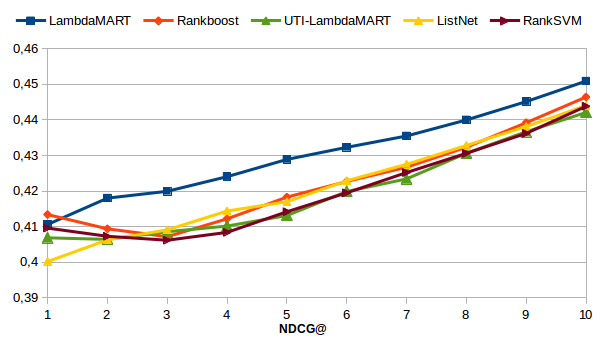
\includegraphics[width=10cm, height=5cm]{im_ndcg_baseline.png}

\caption{Comparison Results with NDCG@1~10 on MQ2007}

\label{fig:ncdg10}

\end{center}

\end{figure}

We also compared the performance of UTI-LambdaMART and BM25 being used
as base rankers combined with LambdaMART as the top ranker. While in
LETOR there is almost no difference between UTI methods and other
learning methods, in practice search engines may contain other
important features available only at query processing times, such as
clicks performed by the users in the top results or personalized
information about each user. Figure~\ref{fig:bm25} compares the
performance of the two alternative base rankers when varying the size
of top results taken from each alternative. As smaller is the number
of top results we need to look in order to achieve high quality
results, as better is the top ranker. As it can be seen,
UTI-LambdaMART outperforms BM25 as a base ranker. For instance, taking
2 results we achieve value of NDCG close to 0.56 when using
UTI-LambdaMART, while to achieve the same quality with BM25 we need to
take 9 top results. With 3 results the UTI base rankers outperform the
results of BM25 as top ranker.

This results is interesting to show how we can employ UTI-LambdaMART
in practical web search scenarios as a base ranker. It reduces the
amount of features to be fetched and computed at query processing
times and reduces the number of top results that should be inspected
by the top ranker when compared to a traditional approach that uses a
simpler base ranker, as BM25. This combination means practical gains
in performance that depend on the architecture and feature sets
adopted by each system.


%\begin{figure}[h!]

%\begin{center}

%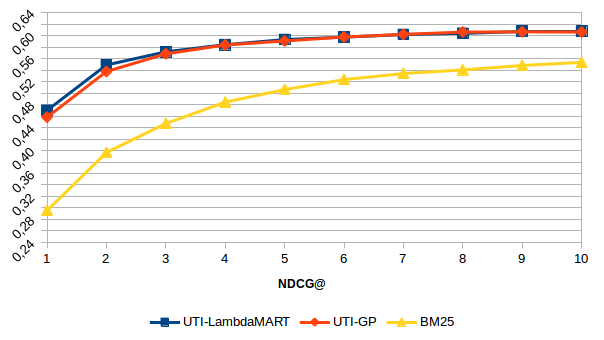
\includegraphics[width=10cm, height=5cm]{im_ndcg10leprefbm25.png}

%\caption{LambdaMART: Comparison results with BM25 base ranker and LePrEF base ranker}

%\label{fig:bm25}

%\end{center}

%\end{figure}


%}


\begin{figure*}[h!]
\centering

\subfigure[LambdaMART: Comparison results with BM25 base ranker and LePrEF base ranker]{
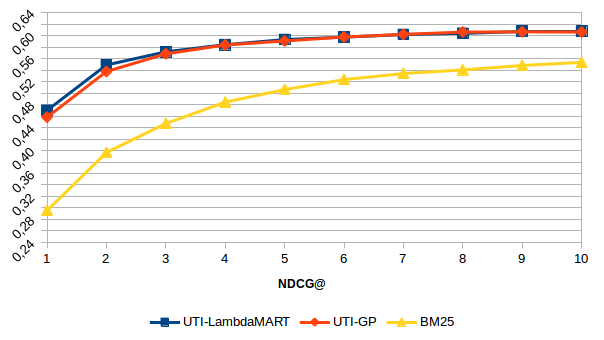
\includegraphics[width=0.5\textwidth]{im_ndcg10leprefbm25.png}
\label{fig:bm25}}

\subfigure[Compression rate achieved by applying Elias-$\delta$ to the UTI values produced by UTI-LambdaMART in the index compared with the NDCG@10;]{
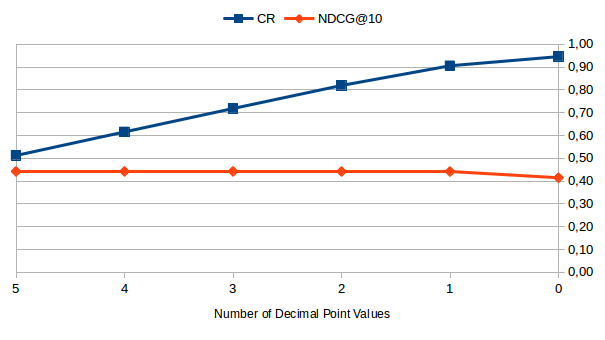
\includegraphics[width=0.5\textwidth]{im_cr_ndcg_lambda.png}
\label{fig:crq}}

\end{figure*}


\subsection{Compressing the UTIs}

\label{sec:compression}


A common approach for improving search engine time and space
efficiency is to compress the inverted
index~\cite{baezaribeiro2011modinforet}. To this effect, we
experimented with truncating the UTI values generated to an integer
value. We performed UTI-LambdaMART with real values and then process
the discretization in final results when storing the inverted list.
This simple strategy achieved satisfactory results with practically no
variation in quality. Without loss of generality, for the experiments
to compress the UTI values, we adopted the \textit{Elias Delta
codes}~\cite{elias1975universal}, a technique that has been adopted
not only in LePrEF, but also in other past research articles that
addressed the topic of compressing inverted indexes.


Figure~\ref{fig:crq} shows the compression rates achieved when varying
the number of digits truncated in the UTI number. As a reference to
compute the compression rate, we adopted that each UTI number would be
represented as a 32 bits floating point number without compression. As
can be seen, there is indeed a trade-off between quality and
compression rate as we vary the number of decimal point values
truncated when transforming real values of UTI into integer values.
Results truncating the number with only $1$ digit presents a small
reduction in NDCG quality while achieves a high compression rate. When
using zero digits, we see a clear negative impact in the NDCG values,
indicating that the best alternative in the experiments with LETOR
would be to truncate UTI values to 1 decimal digit.


%\begin{figure}[h!]

%\begin{center}

%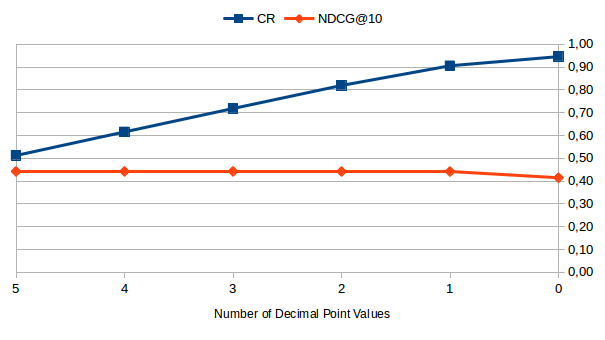
\includegraphics[width=10cm, height=5cm]{im_cr_ndcg_lambda.png}

%\caption{Compression rate achieved by applying Elias-$\delta$ to the UTI values produced by UTI-LambdaMART in the index when (CR) x NDCG@10}

%\label{fig:crq}

%\end{center}

%\end{figure}


%\begin{figure*}[h!]

%\centering

% \subfigure[UTI without compression. 235.234 distinct values. 213.140 unique %values]{%

% 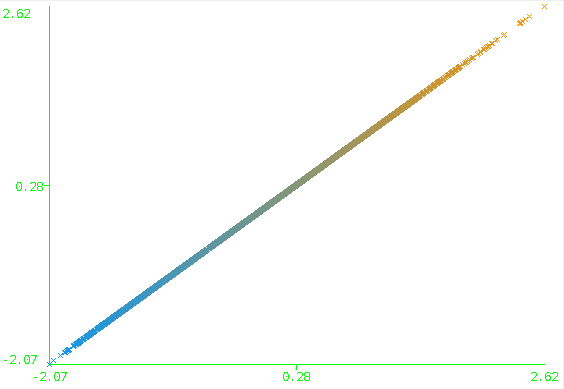
\includegraphics[width=0.4\textwidth]{im_distribuicao_uti_lambda_normal.png}

% \label{fig:dln}}%

% \subfigure[UTI with compression. 47 distinct values; 2 unique values;]{%

% 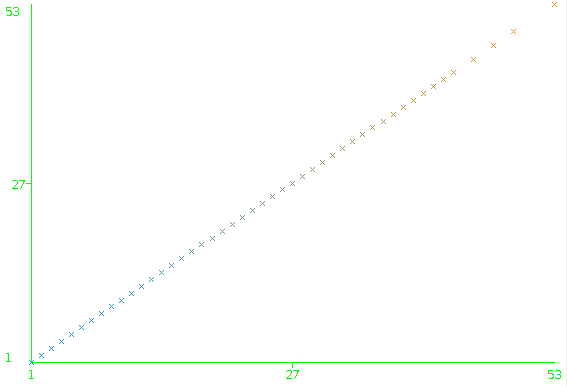
\includegraphics[width=0.4\textwidth]{im_distribuicao_uti_lambda_1casa.png}

% \label{fig:dlc}}

%

% \caption{Distribution of 272.140 UTI values for 5 folds without compression (a) and with compression (b).}

% \label{fig:compareData}

%\end{figure*}



%\begin{figure}

%\begin{center}

%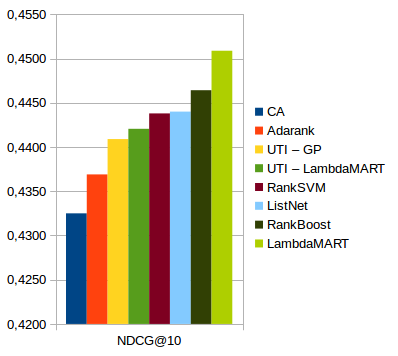
\includegraphics[width=7cm, height=7cm]{im_baselineLePrEF.png}

%\caption{NDCG@10 result obtained by LambdaMART and CA when performed using BM25 and LePrEF as %first ranking.}

%\label{fig:lfr}

%\end{center}

%\end{figure}


%% References

%%

%% Following citation commands can be used in the body text:

%% Usage of \cite is as follows:

%% \cite{key} ==>> [#]

%% \cite[chap. 2]{key} ==>> [#, chap. 2]

%%


%% References with bibTeX database:


\section{Conclusion}

The experimental results presented in this work indicate that
UTI-LambdaMART produces quality results closer to the ones produced by
UTI-GP, while significantly reduces the time required for learning the
model. Further, in the experiments with LETOR, we achieved higher
compression results than those achieved by \cite{costa2012lepref}.


We also investigated two scenarios where UTI values can be used in a
practical web search, considering both, the use of UTI-LambdaMART as
the base ranker and using UTI-LambdaMART as top ranker. In the first,
UTI values are able to produce high quality first cut rankings that
are closer to the final document order, reducing the amount of
documents necessary to be inspected in the top ranker, and resulting
in gains of performance. In the second scenario, UTI-LambdaMART is
directly applied as the top ranker, and we show that, even taking only
features available at indexing times, it produces rankings with
quality closer to learn to rank methods adopted at query processing
times, but with the advantage of adopting a very simple ranking
strategy at query processing times.


\label{conclusion}



\bibliographystyle{elsarticle-num}

% \bibliographystyle{elsarticle-harv}

% \bibliographystyle{elsarticle-num-names}

% \bibliographystyle{model1a-num-names}

% \bibliographystyle{model1b-num-names}

% \bibliographystyle{model1c-num-names}

% \bibliographystyle{model1-num-names}

% \bibliographystyle{model2-names}

% \bibliographystyle{model3a-num-names}

% \bibliographystyle{model3-num-names}

% \bibliographystyle{model4-names}

% \bibliographystyle{model5-names}

% \bibliographystyle{model6-num-names}


\bibliography{sample}


\end{document}

%%
%% End of file `elsarticle-template-num.tex'.
